% SPDX-License-Identifier: CC-BY-SA-4.0
% Author: Matthieu Perrin
% Part: 
% Section: 
% Sub-section: 
% Frame: 

\begingroup

\subsection{Analyse syntaxique}

\begin{frame}{Statégie d'analyse syntaxique}
  \begin{block}{Algorithme Cocke-Younger-Kasami (CYK)}

    \begin{description}
    \item [Entrées]
      \begin{itemize}
      \item Une grammaire algébrique $G = \langle \Sigma, \Gamma, S, R \rangle$ \\ sous \structure{forme normale de Chomsky}
      \item Un mot $u$
      \end{itemize}

    \item [Sortie :] Une réponse booléenne sur \structure{$u \in \mathcal{L}(G)$}

    \item [Complexité :] $\mathcal{O}\left(|R| \times |u|^3 \right)$
    \end{description}
  \end{block}
\end{frame}

\begin{frame}{Forme normale de Chomsky}
  
  \begin{block}{Forme normale de Chomsky}
    Soit $G = \langle \Sigma, \Gamma, S, R \rangle$ une grammaire algébrique.

    $G$ est en \structure{forme normale de Chomsky} si les règles de $R$ sont de la forme :
    \begin{enumerate}
    \item $N \rightarrow XY$ \hspace{5mm} avec $N\in \Gamma$ et $X, Y \in \Gamma$
    \item $N \rightarrow a$  \hspace{8mm} avec $N \in \Gamma$ et $a\in \Sigma$
    \end{enumerate}
    ou bien toutes ses règles sont de la forme :
    \begin{enumerate}
    \item $N \rightarrow XY$ \hspace{5mm} avec $N\in \Gamma$ et $X, Y \in \Gamma \setminus \{S\}$
    \item $N \rightarrow a$  \hspace{8mm} avec $N \in \Gamma$ et $a\in \Sigma$
    \item $S \rightarrow \varepsilon$
    \end{enumerate}
  \end{block}

  \begin{block}{Théorème}
    Toute grammaire algébrique peut être transformée en une
    grammaire en \structure{forme normale de Chomsky} reconnaissant le même langage. 
  \end{block}
\end{frame}

\begin{frame}{Transformation en forme normale de Chomsky}\label{slide:FNC}

  \begin{block}{Démonstration du théorème}
    Appliquer successivement les règles suivantes :
    \begin{enumerate}
    \item Introduire une règle \structure{$X \rightarrow x$} pour chaque $x\in \Sigma$
    \item Eliminer les règles \structure{$X \rightarrow ...S...$} 
    \item Eliminer les règles \structure{$X \rightarrow \varepsilon$} pour $X \not= S$
    \item Eliminer les règles \structure{$X \rightarrow Y$}
    \item Remplacer les règles \structure{$N \rightarrow A_1 A_2 ... A_n$} par \structure{$N \rightarrow A_1 B$} et \structure{$B \rightarrow A_2 ... A_n$}
    \end{enumerate}
  \end{block}

  \begin{exampleblock}{Exemple}
    \scalebox{.9}{
      \begin{tikzpicture}
        \draw[white] (-2.5,1) rectangle (8.5,5);
        \draw (0,5) node[below]{\begin{minipage}{.45\textwidth}
            $\left\{
            \only<1>{\begin{array}{lll}
                S &\rightarrow& aSb \;|\; T \\
                T &\rightarrow& cT \;|\; \varepsilon\\
            \end{array}}
            \only<2>{\begin{array}{lll}
                S &\rightarrow& \alert{a}S\alert{b} \;|\; T \\
                T &\rightarrow& \alert{c}T \;|\; \varepsilon\\
            \end{array}}
            \only<3>{\begin{array}{lll}
                S &\rightarrow& A\alert{S}B \;|\; T \\
                T &\rightarrow& CT \;|\; \varepsilon\\
                A &\rightarrow& a  \\
                B &\rightarrow& b\\
                C &\rightarrow& c \\
            \end{array}}
            \only<4>{\begin{array}{lll}
                S &\rightarrow& D \\
                D &\rightarrow& ADB \;|\; T \\
                T &\rightarrow& CT \;|\; \alert{\varepsilon} \\
                A &\rightarrow& a \\
                B &\rightarrow& b \\
                C &\rightarrow& c \\
            \end{array}}
            \only<5>{\begin{array}{lll}
                S &\rightarrow& D \\
                D &\rightarrow& ADB \;|\; T \;|\; \alert{\varepsilon} \\
                T &\rightarrow& CT \;|\; C \\
                A &\rightarrow& a \\
                B &\rightarrow& b \\
                C &\rightarrow& c \\
            \end{array}}
            \only<6>{\begin{array}{lll}
                S &\rightarrow& \alert{D} \;|\; \varepsilon \\
                D &\rightarrow& ADB  \;|\; AB \;|\; \alert{T} \\
                T &\rightarrow& CT \;|\; \alert{C} \\
                A &\rightarrow& a \\
                B &\rightarrow& b \\
                C &\rightarrow& c \\
            \end{array}}
            \only<7>{\begin{array}{lll}
                S &\rightarrow& \alert{ADB}  \;|\; AB \;|\; CT \;|\; c \;|\; \varepsilon \\
                D &\rightarrow& \alert{ADB}  \;|\; AB \;|\; CT \;|\; c \\
                T &\rightarrow& CT \;|\; c \\
                A &\rightarrow& a \\
                B &\rightarrow& b \\
                C &\rightarrow& c \\
            \end{array}}
            \only<8>{\begin{array}{lll}
                S &\rightarrow& AE  \;|\; AB \;|\; CT \;|\; c \;|\; \varepsilon \\
                D &\rightarrow& AE  \;|\; AB \;|\; CT \;|\; c \\
                E &\rightarrow& DB \\
                T &\rightarrow& CT \;|\; c \\
                A &\rightarrow& a \\
                B &\rightarrow& b \\
                C &\rightarrow& c \\
            \end{array}}
            \right.$
        \end{minipage}};
        \draw (6.5,5) node[below]{\begin{minipage}{.58\textwidth}
            \only<2>{
              Application de la règle 1.
              \begin{enumerate}
              \item Introduire trois nouveaux non-terminaux\\ $A$, $B$ et $C$ 
              \item Introduire les règles
                \\$A \rightarrow a$, $B \rightarrow b$, $C \rightarrow c$
              \item Remplacer $a$ par $A$, $b$ par $B$ et $c$ par $C$
                %\item Remplacer les terminaux\\ $aSb$ par $ASB$ et $cT$ par $CT$
              \end{enumerate}
            }
            \only<3>{
              Application de la règle 2.
              \begin{enumerate}
              \item Introduire un nouveau non-terminal $D$ 
              \item Renommer $S$ en $D$
              \item Introduire une règle $S \rightarrow D$
              \end{enumerate}
            }
            \only<4>{
              Application de la règle 3.
              \begin{enumerate}
              \item Isoler $\varepsilon$ dans $T$ :\\
                $\begin{array}{lll}
                T &\rightarrow& T' \;|\; \varepsilon\\
                T' &\rightarrow& CT\\
              \end{array}$

              \item Remplacer $T$ par sa définition $T' \;|\; \varepsilon$
              \item Renommer $T'$ en $T$
              \end{enumerate}
            }
            \only<5>{
              Application de la règle 3 à nouveau.
              \begin{enumerate}
              \item Isoler $\varepsilon$ dans $D$ :\\
                $\begin{array}{lll}
                D &\rightarrow& D' \;|\; \varepsilon\\
                D' &\rightarrow& ABD\;|\; T\\
              \end{array}$

              \item Remplacer $D$ par sa définition $D' \;|\; \varepsilon$
              \item Renommer $D'$ en $D$
              \end{enumerate}
            }
            \only<6>{
              Application de la règle 4.
              \begin{enumerate}
              \item Remplacer $T \rightarrow C$ par $T \rightarrow c$
              \item Remplacer $D \rightarrow T$ par $D \rightarrow CT \;|\; c$
              \item Remplacer $S \rightarrow D$ par $S \rightarrow ADB  \;|\; AB \;|\; CT \;|\; c$
              \end{enumerate}
            }
            \only<7>{
              Application de la règle 5.
              \begin{enumerate}
              \item Remplacer $S \rightarrow ADB$ par :\\
                $\begin{array}{lll}
                S &\rightarrow& AE\\
                E &\rightarrow& BD\\
              \end{array}$
              \end{enumerate}
            }
        \end{minipage}};
    \end{tikzpicture}}
  \end{exampleblock}
\end{frame}


\begin{frame}[fragile]{Algorithme Cocke-Younger-Kasami (CYK)}
  \begingroup
  \renewcommand{\emph}[1]{\structure{#1}} 
  \vspace{-1mm}
  
  ~\hspace{-5mm}
  \begin{tikzpicture}

    \fill<2>[rounded corners,alert!20] (-1.1,3.35) rectangle (0.4,3.65);
    \fill<3>[rounded corners,alert!20] (-1.8,5.25) rectangle (1.9,5.6);
    \fill<4->[rounded corners,alert!20] (-1.4,3.8) rectangle (6.1,4.6);

    \draw (5,4.85) node{\begin{minipage}{15cm}\scalebox{.7}{\begin{algorithm}[H]
            \SetKwFunction{CYK}{CYK}
            \SetKwData{Input}{motif}
            
            \Fn{\CYK($\langle \Sigma, \Gamma, S, R \rangle$ : grammaire, $u \in \Sigma^\star$) : booléen}{
              \lSi{$u = \varepsilon$}{\Retourner $S \rightarrow \varepsilon \in R$}
              \Pour{$j$ allant de $1$ à $|u|$}{
                $T[1, j] \leftarrow \{N\in \Gamma | N \rightarrow u[j] \in R\}$\;
              }
              \Pour{$i$ allant de $2$ à $|u|$}{
                \Pour{$j$ allant de $1$ à $|u|-i+1$}{
                  $\displaystyle T[i, j] \leftarrow \bigcup_{k=1}^{i-1} \{N\in \Gamma | \exists X \in T[k,j], \exists Y \in T[i-k,j+k], N \rightarrow X Y \in R\}$\;
                }
              }
              \Retourner $S\in T[|u|, 1]$\;
            }
    \end{algorithm}}\end{minipage}};

    \draw (0,1.5) node{\footnotesize\begin{minipage}{4.7cm}\begin{exampleblock}{Exemple}

        \vspace{2mm}
        $G=\left\{\begin{array}{lll}
        \alert<5,9>{S} &\alert<5,9>{\rightarrow}&  \alert<9>{AC} \;|\; \alert<5>{AB} \;|\; \varepsilon  \\
        \alert<8>{C} &\alert<8>{\rightarrow}&  \alert<8>{TB}  \\
        \alert<5,9>{T} &\alert<5,9>{\rightarrow}&  \alert<9>{AC} \;|\; \alert<5>{AB}  \\
        \alert<3>{A} &\alert<3>{\rightarrow}& \alert<3>{a}  \\
        \alert<3>{B} &\alert<3>{\rightarrow}& \alert<3>{b} \end{array}\right.$

        \vspace{2mm}
        $u = aabb$
      \end{exampleblock}\end{minipage}
    };
    
    \draw (5.4,0.8) node{
      \begin{tikzpicture}
        \draw[white] (-.75,-1) rectangle (6,2.8);
        \draw (-.75,2.8) node[above left]{\scriptsize $T[i,j]$};
        \draw (0.0 ,2.8) node[above]{\scriptsize $j=1$};
        \draw (1.5 ,2.8) node[above]{\scriptsize $j=2$};
        \draw (3.0 ,2.8) node[above]{\scriptsize $j=3$};
        \draw (4.5 ,2.8) node[above]{\scriptsize $j=4$};
        \draw (-.75,2.4) node[left] {\scriptsize $i=1$};
        \draw (-.75,1.6) node[left] {\scriptsize $i=2$};
        \draw (-.75,0.8) node[left] {\scriptsize $i=3$};
        \draw (-.75,0.0) node[left] {\scriptsize $i=4$};


        \draw[fill=structure!15] (0.0,2.4) +(-.75,-.4) node[above right]{\footnotesize \example{$a$}}    rectangle +(.75,.4) +(0,.15) node{\only<2>{$\structure{\{...\}}$}\only<3->{\alert<3>{$\{A\}$}}};
        \draw[fill=structure!15] (1.5,2.4) +(-.75,-.4) node[above right]{\footnotesize \example{$a$}}    rectangle +(.75,.4) +(0,.15) node{\only<2>{$\structure{\{...\}}$}\only<3->{\alert<3>{$\{A\}$}}};
        \draw[fill=structure!15] (3.0,2.4) +(-.75,-.4) node[above right]{\footnotesize \example{$b$}}    rectangle +(.75,.4) +(0,.15) node{\only<2>{$\structure{\{...\}}$}\only<3->{\alert<3>{$\{B\}$}}};
        \draw[fill=structure!15] (4.5,2.4) +(-.75,-.4) node[above right]{\footnotesize \example{$b$}}    rectangle +(.75,.4) +(0,.15) node{\only<2>{$\structure{\{...\}}$}\only<3->{\alert<3>{$\{B\}$}}};
        \draw[fill=structure!15] (0.0,1.6) +(-.75,-.4) node[above right]{\footnotesize \example{$aa$}}   rectangle +(.75,.4) +(0,.15) node{\only<2>{$\structure{\{...\}}$}\only<4->{\alert<4>{$\emptyset$}}};
        \draw[fill=structure!15] (1.5,1.6) +(-.75,-.4) node[above right]{\footnotesize \example{$ab$}}   rectangle +(.75,.4) +(0,.15) node{\only<2>{$\structure{\{...\}}$}\only<5->{\alert<5>{$\{S, T\}$}}};
        \draw[fill=structure!15] (3.0,1.6) +(-.75,-.4) node[above right]{\footnotesize \example{$bb$}}   rectangle +(.75,.4) +(0,.15) node{\only<2>{$\structure{\{...\}}$}\only<6->{\alert<6>{$\emptyset$}}};
        \draw[fill=structure!15] (0.0,0.8) +(-.75,-.4) node[above right]{\footnotesize \example{$aab$}}  rectangle +(.75,.4) +(0,.15) node{\only<2>{$\structure{\{...\}}$}\only<7->{\alert<7>{$\emptyset$}}};
        \draw[fill=structure!15] (1.5,0.8) +(-.75,-.4) node[above right]{\footnotesize \example{$abb$}}  rectangle +(.75,.4) +(0,.15) node{\only<2>{$\structure{\{...\}}$}\only<8->{\alert<8>{$\{C\}$}}};
        \draw[fill=structure!15] (0.0,0.0) +(-.75,-.4) node[above right]{\footnotesize \example{$aabb$}} rectangle +(.75,.4) +(0,.15) node{\only<2>{$\structure{\{...\alert{S?}...\}}$}\only<9->{$\{\alert{S}, T\}$}};

        \draw<1>[-latex, example] (1.25,0.9) -- (1.25,2.5);
        \draw<1>[-latex, example] (1.25,0.9) -- (4.25,2.5);

        \draw<1,2> (2.25,1.2) node[below right]{\begin{minipage}{3.2cm}\footnotesize
            \example{$T[i,j]$ représente le facteur \\$u_{i,j} = u[j], ..., u[j+i]$ }
        \end{minipage}};
        \draw<2> (2.25,0) node[right]{\begin{minipage}{3.2cm}\footnotesize \structure{$T[i,j]$ contient \\ $\{N \in \Gamma | N \vdash^\star u_{i,j}\}$ }\end{minipage}};

        \draw<4> (2.25,1.2) node[below right]{\begin{minipage}{3.2cm}\footnotesize
            On cherche \alert{$N \rightarrow XY \vdash aa$}\\
            $\bullet$ $X = A \in T[1,1]$ \\
            $\bullet$ $Y = A \in T[1,2]$ \\
            Pas de règle \alert{$N \rightarrow AA$}\\
        \end{minipage}};

        \draw<5> (2.25,1.2) node[below right]{\begin{minipage}{3.2cm}\footnotesize
            On cherche \alert{$N \rightarrow XY \vdash ab$}\\
            $\bullet$ $X = A \in T[1,2]$ \\
            $\bullet$ $Y = B \in T[1,3]$ \\
            Deux règles \alert{$N \rightarrow AB$}\\
        \end{minipage}};

        \draw<6> (2.25,1.2) node[below right]{\begin{minipage}{3.2cm}\footnotesize
            On cherche \alert{$N \rightarrow XY \vdash bb$}\\
            $\bullet$ $X = B \in T[1,3]$ \\
            $\bullet$ $Y = B \in T[1,4]$ \\
            Pas de règle \alert{$N \rightarrow BB$}\\
        \end{minipage}};

        \draw<7> (2.25,1.2) node[below right]{\begin{minipage}{3.5cm}\footnotesize
            $aab = a \cdot ab = aa \cdot b$\\
            On cherche \alert{$N \rightarrow XY$}\\
            $\bullet$ $X \vdash^\star a$, $Y \vdash^\star ab$  \\
            $\bullet$ $X \vdash^\star aa$, $Y \vdash^\star b$  \\
            \scriptsize \alert{$XY \in \{A\} \cdot \{S, T\} \cup \emptyset \cdot \{B\}$}\\
            Pas de règle \alert{$N \rightarrow AS$} ou \alert{$N \rightarrow AT$}\\
        \end{minipage}};
        \draw<7>[alert] (0.0,2.55)  -- (1.5,1.75);
        \draw<7>[alert] (0.0,1.75)  -- (3.0,2.55);

        \draw<8> (2.25,1.2) node[below right]{\begin{minipage}{3.5cm}\footnotesize
            $aab = a \cdot bb = ab \cdot b$\\
            On cherche \alert{$N \rightarrow XY$}\\
            $\bullet$ $X \vdash^\star a$, $Y \vdash^\star bb$  \\
            $\bullet$ $X \vdash^\star ab$, $Y \vdash^\star b$  \\
            \scriptsize \alert{$XY \in \{A\} \cdot \emptyset \cup \{S, T\} \cdot \{B\}$}\\
            Une règle \alert{$N \rightarrow TB$}\\
        \end{minipage}};

        \draw<8>[alert] (1.5,2.55)  -- (3.0,1.75);
        \draw<8>[alert] (1.5,1.75)  -- (4.5,2.55);

        \draw<9> (2.25,1.2) node[below right]{\begin{minipage}{3.5cm}\footnotesize
            $\begin{array}{lll}aabb &=& a \cdot bbb \\ &=& aa \cdot bb\\ &=& aab \cdot b\\ \alert{aabb} & \alert{\in} &\alert{\mathcal{L}(G)}\end{array}$\\
        \end{minipage}};

        \draw<9>[alert] (0,2.55)  -- (1.5,0.95)  ;
        \draw<9>[alert] (0,1.75)  -- (3.0,1.75)  ;
        \draw<9>[alert] (0,0.95)  -- (4.5,2.55)  ;

      \end{tikzpicture}
    };
  \end{tikzpicture}
  \endgroup
\end{frame}

\subsection{Automates à pile}

\begin{frame}{Automates finis généralisés}

  \begin{block}{Automate fini généralisé}

    Si un automate fini n'est pas suffisant, ajouter une structure de données
    \begin{itemize}
    \item Pile : \structure{automate à pile}
    \item\vspace{-1mm} Tableau de taille $|u|$ : \structure{machine linéairement bornée}
    \item\vspace{-1mm} Ruban infini : \structure{machine de Turing}
    \end{itemize}
  \end{block}
  \begin{exampleblock}{Exemple : le langage $\{a^n b^n | n>0\}$}
    \vspace{-1mm}
    \begin{tikzpicture}
      \draw (5,5) node[below]{\begin{minipage}{\textwidth}%
          \begin{algorithm}[H]
            \SetKwFunction{Dick}{decide}
            \Fn{$\Dick(u : \text{mot}) : \text{booléen}$}{
              $q\leftarrow 0$; $c \leftarrow 0$\;
              \Pour{$i$ allant de $1$ à $|u|$}{
                \uSi{$q = 0 \land u[i] = \text{`$a$'}$}{
                  $c \leftarrow c + 1$
                }
                \uSinonSi{$c > 0 \land u[i] = \text{`$b$'}$}{
                  $q\leftarrow 1$;
                  $c \leftarrow c - 1$\;
                }
                \lSinon{\Retourner \False}
              }
              \Retourner $q=1 \land c=0$\;
            }
          \end{algorithm}
      \end{minipage}};
      
      \draw (8.5,4.8) node[below]{\begin{minipage}{4cm}\structure{Grammaire :}

          \vspace{2mm}
          $S \rightarrow a S b \,|\, ab $\\
          
          \structure{Automate à compteur :}
          
          \vspace{2mm}
          \begin{tikzpicture}[shorten >=1pt,node distance=2cm,on grid,auto]
            \node[state, initial, initial text=] (a)              {0};
            \node[state, accepting]              (b) [right=of a] {1};
            \path[->] (a) edge[loop above, looseness=5] node {$a / c\text{++}$} (a);
            \path[->] (a) edge node {$b / c\text{-\,-}$} (b);
            \path[->] (b) edge[loop above, looseness=5] node {$b / c\text{-\,-}$} (b);
          \end{tikzpicture}
      \end{minipage}};
    \end{tikzpicture}
  \end{exampleblock}
\end{frame}

\begin{frame}[fragile]{Algorithme de reconnaissance récursif}
  \vspace{-3mm}
  
  ~\hspace{-5mm}
  \begin{tikzpicture}
    
    \draw[white] (-.5,-.9) rectangle (11.7,7.3);
    
    \draw (8.5,4.8) node[right]{\begin{minipage}{4cm}\begin{block}{Grammaire}
          $\left\{\begin{array}{l}
          S \rightarrow \varepsilon\\
          S \rightarrow \alert{\{}S\alert{\}}S\\
          S \rightarrow \hspace{.2mm}\alert{\langle}\hspace{.2mm}S\hspace{.2mm}\alert{\rangle}\hspace{.2mm}S\\
          \end{array}\right.$
    \end{block}\end{minipage}};
    \draw (5,5) node{\begin{minipage}{\textwidth}\scalebox{1}{\begin{algorithm}[H]
            \SetKwFunction{Decider}{decider}
            \SetKwFunction{Trouver}{S}
            \Fn{$\Decider(u : \text{mot}) : \text{booléen}$}{
              \Retourner $\Trouver( u \cdot \text{`$\diamond$'}, \text{`$\diamond$'} )$\;
            }
            \Fn{$\Trouver(\textbf{\color{black}m } u : \text{mot}, \omega : \text{caractère}) : \text{booléen}$}{
              \lSi{$u = \varepsilon$}{\Retourner \False}
              $c \leftarrow u[1]$; 
              $u \leftarrow u[2]...u[|u|]$\;
              \lSi{$c = \omega\,$}{\Retourner \True}
              \lSi{$c = \alert{\text{`$\{$'}}$}{\Retourner $\Trouver(u, \alert{\text{`$\}$'}}) \land \Trouver(u, c)$}
              \lSi{$c = \hspace{.3mm}\alert{\text{`$\langle$'}}$}{\Retourner $\Trouver(u, \alert{\text{`$\rangle$'}}) \land \Trouver(u, c)$}
              \Retourner \False\;
            }
    \end{algorithm}}\end{minipage}};
    
    \draw<2-> (1.5,2.2) node{
      \begin{minipage}{3cm}
        \begin{exampleblock}{Exemple}
          $\phantom{\{\langle\}}u = \only<-3>{\{}\only<-4>{\{}\only<-5>{\}}\only<-6>{\langle}\only<-7>{\rangle}\only<-8>{\}}\only<3-9>{\diamond}\only<10>{\varepsilon}$
        \end{exampleblock}
      \end{minipage}
    };

    \draw<2-> (6.2,1) node{\begin{minipage}{6cm}
        \begin{tikzpicture}[shorten >=1pt,node distance=1.5cm,on grid,auto]

          \draw (-1,2) -- (-1,-.25) -- ( 1,-.25) -- ( 1,2);
          \draw (-1,0.25) -- ( 1,0.25);
          \draw (-1,0.75) -- ( 1,0.75);
          \draw (-1,1.25) -- ( 1,1.25);
          \draw (-1,1.75) -- ( 1,1.75);
          
          \draw<7> (0,1.5)   node{$\Trouver(u, \rangle)$};
          \draw<5> (0,1.5)   node{$\Trouver(u, \})$};
          \draw<4-8> (0,1.0) node{$\Trouver(u, \})$};        \draw<6-8> (.85,.85) node{\tiny \only<-7>{$\times 2$}\only<8->{$\times 3$}};
          \draw<3-9> (0,0.5) node{$\Trouver(u, \diamond)$};
          \draw<2-> (0,0.0)  node{$\Decider(u)$};
        \end{tikzpicture}
    \end{minipage}};

    \draw<3-> (7.2,1) node{\begin{minipage}{3cm}
        \begin{tikzpicture}[shorten >=1pt,node distance=1.5cm,on grid,auto]
          \node[state, initial above, initial text=$\text{empile}(\diamond)$] (a) {0};
          \uncover<10->{
            \node[state, accepting] (b) [below=of a] {1};
          }
          
          \path [->] (a) edge [loop right, looseness=5] node {$\begin{array}{rcl}
              \uncover<7->{\langle &:& \text{empile}(\langle)}\\
              \uncover<4->{\{ &:& \text{empile}(\})}\\
              \uncover<6->{\} &:& \text{dépile}(\})}\\
              \uncover<8->{\rangle &:& \text{dépile}(\rangle)}\\
            \end{array}$} (a);

          \uncover<10->{
            \path [->] (a) edge node [left]{$\diamond : \text{dépile}(\diamond)$} (b);
          }
          
        \end{tikzpicture}
    \end{minipage}};
  \end{tikzpicture}
\end{frame}


\begin{frame}{Modélisation mathématique}
  \vspace{-10mm}
  \begin{block}{Définition -- Automate à pile non-déterministe}
    Un \structure{automate à pile} est un septuplet \alert{$\langle \Sigma, \Pi, Q, I, F, \diamond, \mu \rangle$} tel que :
    \begin{description}
    \item[\alert{$\Sigma$}] ensemble fini non vide : \structure{l'alphabet d'entrée}
    \item[\alert{$\Pi$}] ensemble fini non vide : \structure{l'alphabet de pile}
    \item[\alert{$Q$}] ensemble fini non vide : \structure{les états possibles}
    \item[\alert{$I$}] $\subseteq Q$ : \structure{les états initiaux}
    \item[\alert{$F$}] $\subseteq Q$ : \structure{les états finaux (ou accepteurs)}
    \item[\alert{$\diamond$}] $\in \Pi$ : \structure{le symbole de fond de pile}
    \item[\alert{$\mu$}] $\subseteq  (Q \times \Sigma^\star \times \Pi^\star) \times (Q \times \Pi^\star)$ : \structure{la relation de transition}
    \end{description}

    Une \structure{transition} est un tuple \alert{$\langle \langle q, u, p \rangle, \langle q', p' \rangle \rangle \in \mu$} tel que :
    \begin{description}
    \item[\alert{$q$}] $\in Q$ : \structure{l'état de départ}
    \item[\alert{$u$}] $\in \Sigma^\star$ : \structure{le mot reconnu}
    \item[\alert{$p$}] $\in \Pi^\star$ : \structure{le mot dépilé}
    \item[\alert{$q'$}] $\in Q$ : \structure{l'état d'arrivée}
    \item[\alert{$p'$}] $\in \Pi^\star$ : \structure{le mot empilé}
    \end{description}
  \end{block}

  \vspace{-2cm}\hspace{7cm}  \scalebox{.9}{\begin{tikzpicture}[shorten >=1pt,node distance=1.5cm,on grid,auto]
      \node [state] (q) {$q$}; 
      \node         (a) [right=of q]  {}; 
      \node [state] (q1) [right=of a]  {$q'$}; 
      \path [->]    (q) edge node {$u / p / p'$} (q1);
  \end{tikzpicture}}
\end{frame}

\begin{frame}{Configurations et actions d'un automate à pile}
  Soit $A=\langle \Sigma, \Pi, Q, I, F, \diamond, \mu \rangle$ un automate à pile. 
  
  \begin{block}{Définition -- configuration}
    Une \structure{configuration} de $A$ est un triplet \alert{$\langle u, q, \pi \rangle$} tel que :
    \begin{description}
    \item[\alert{$u$}] $\in \Sigma^\star$ : \structure{mot restant à reconnaître}
    \item[\alert{$q$}] $\in Q$ : \structure{l'état courant dans la simulation}
    \item[\alert{$\pi$}] $\in \Pi^\star$ : \structure{l'état courant de la pile}
    \end{description}
  \end{block}

  \begin{block}{Définition -- action et chemin d'actions}
    Les \structure{actions} de $A$ sont définies par une
    relation binaire \alert{$\leadsto_A$} sur les configurations.
    Pour tous $u, v \in \Sigma^\star$, $\pi, p, p' \in \Pi^\star$, $q, q'\in Q$, on a 
    \alert{$$\langle v \cdot u, q, p \pi \rangle \leadsto_A \langle u, q', p' \pi \rangle \hspace{3mm} \Leftrightarrow \hspace{3mm} \langle \langle q, v, p \rangle, \langle q', p' \rangle \rangle \in \mu$$}
    On note \alert{$\leadsto_A^\star$} la fermeture transitive et réflexive de $\leadsto_A$.
  \end{block}
\end{frame}

\begin{frame}{Langages reconnus par un automate à pile}
  \small
  
  Soit $A=\langle \Sigma, \Pi, Q, I, F, \diamond, \mu \rangle$ un automate à pile.

  \begin{block}{Définition -- langage reconnu}
    \begin{itemize}
    \item\vspace{-1mm} Le \structure{langage des mots reconnus par état final}, noté $\alert{\mathcal{L}_F(A)}$ est l'ensemble des mots menant d'un état initial à un état final, quelle que soit la pile à l'arrivée. 
      $$\alert{\mathcal{L}_F(A) = \{u \in \Sigma^\star | \exists i\in I, \exists \structure{f\in F}, \exists \structure{\pi\in\Pi^\star}, \langle u, i, \diamond \rangle \leadsto_A^\star \langle \varepsilon, \structure{f}, \structure{\pi} \rangle\}}$$
    \item\vspace{-1mm} Le \structure{langage des mots reconnus par pile vide}, noté $\alert{\mathcal{L}_\varepsilon(A)}$ est l'ensemble des mots menant d'un état initial à un état quelconque et une pile vide. 
      $$
      \alert{\mathcal{L}_\varepsilon(A) = \{u \in \Sigma^\star | \exists i\in I, \exists \structure{q\in Q}, \langle u, i, \diamond \rangle \leadsto_A^\star \langle \varepsilon, \structure{q}, \structure{\varepsilon} \rangle\}}
      $$
    \item\vspace{-1mm} Le \structure{langage des mots reconnus par état final et pile vide}, noté $\alert{\mathcal{L}(A)}$ est l'ensemble des mots menant d'un état initial à un état final et une pile vide. 
      $$
      \alert{\mathcal{L}(A) = \{u \in \Sigma^\star | \exists i\in I, \exists \structure{f\in F}, \langle u, i, \diamond \rangle \leadsto_A^\star \langle \varepsilon, \structure{f}, \structure{\varepsilon} \rangle\}}
      $$
    \end{itemize}
  \end{block}

  \vspace{-2mm}
  \begin{block}{Équivalence entre méthodes de reconnaissance}
    \begin{itemize}
    \item \vspace{-2mm}Preuve en TD
    \end{itemize}
  \end{block}
  
\end{frame}

\begin{frame}{Exemple : le langage $\{a^n b^n | n\in \mathbb{N}\}$}

  \centering
  \begin{tikzpicture}
    \draw (6,12.5) node{\scalebox{.7}{$\left\langle \{a, b\}, \{A, \diamond\}, \{0, 1, 2\}, \{0\}, \{2\},  \diamond, \left\{
        \begin{array}{cccccccc}
          \langle \langle &0, & a          , & \varepsilon & \rangle, \langle & 0, & A           & \rangle \rangle \\ 
          \langle \langle &0, & b          , & A           & \rangle, \langle & 1, & \varepsilon & \rangle \rangle \\        
          \langle \langle &0, & \varepsilon, & \diamond    & \rangle, \langle & 2, & \varepsilon & \rangle \rangle \\        
          \langle \langle &1, & b          , & A           & \rangle, \langle & 1, & \varepsilon & \rangle \rangle \\        
          \langle \langle &1, & \varepsilon, & \diamond    & \rangle, \langle & 2, & \varepsilon & \rangle \rangle \\        
        \end{array}
        \right\} \right\rangle$}};

    \draw (2,10) node{\begin{tikzpicture}
        \fill<3>  [structure!20] (-.5,0.75) rectangle ( .5,1.25);
        \fill<2-4>[structure!20] (-.5,0.25) rectangle ( .5,0.75);
        \fill<-5> [structure!20] (-.5,-.25) rectangle ( .5,0.25);

        \draw (-.5,2)    -- (-.5,-.25) -- ( .5,-.25) -- ( .5,2);
        \draw (-.5,0.25) -- ( .5,0.25);
        \draw (-.5,0.75) -- ( .5,0.75);
        \draw (-.5,1.25) -- ( .5,1.25);
        \draw (-.5,1.75) -- ( .5,1.75);
        
        \draw<3>   (0,1.0) node{$A$};
        \draw<2-4> (0,0.5) node{$A$};
        \draw<1-5> (0,0.0) node{$\diamond$};
    \end{tikzpicture}};
    
    \draw (8,10) node {\begin{tikzpicture}[shorten >=1pt,node distance=2.5cm,on grid,auto]
        \node [state,initial, initial text=$\diamond$] (a)              {$0$}; 
        \node [state]                        (b) [right=of a] {$1$}; 
        \node [state, accepting]             (c) [right=of b] {$2$}; 

        \node<-3>  [structure, fill=structure!20, state,initial, initial text=] (a)              {$0$}; 
        \node<4-5> [structure, fill=structure!20, state]                        (b) [right=of a] {$1$}; 
        \node<6>   [structure, fill=structure!20, state, accepting]             (c) [right=of b] {$2$}; 

        \path        [->]           (a) edge[bend right]              node[below] {$\varepsilon/\diamond/\varepsilon$} (c);
        \path<1,4->  [->]           (a) edge[loop above, looseness=5] node        {$a/\varepsilon/A$}                  (a);
        \path<2,3>   [structure,->] (a) edge[loop above, looseness=5] node        {$a/\varepsilon/A$}                  (a);
        \path<-3,5-> [->]           (a) edge                          node[above] {$b/A/\varepsilon$}                  (b);
        \path<4>     [structure,->] (a) edge                          node[above] {$b/A/\varepsilon$}                  (b);
        \path<-4,6>  [->]           (b) edge[loop above, looseness=5] node        {$b/A/\varepsilon$}                  (b);
        \path<5>     [structure,->] (b) edge[loop above, looseness=5] node        {$b/A/\varepsilon$}                  (b);
        \path<-5>    [->]           (b) edge                          node[above] {$\varepsilon/\diamond/\varepsilon$} (c);
        \path<6>     [structure,->] (b) edge                          node[above] {$\varepsilon/\diamond/\varepsilon$} (c);
    \end{tikzpicture}};

    \draw (6,7) node{$\begin{array}{rcl}
        \structure<1>{\langle aabb, 0, \diamond \rangle} \uncover<2->{&\leadsto& \structure<2>{\langle abb, 0, A\diamond \rangle}\\}
        \uncover<3->{&\leadsto& \structure<3>{\langle bb, 0, AA\diamond \rangle}\\}
        \uncover<4->{&\leadsto& \structure<4>{\langle b, 1, A\diamond \rangle}\\}
        \uncover<5->{&\leadsto& \structure<5>{\langle \varepsilon, 1, \diamond \rangle}\\}
        \uncover<6->{&\leadsto& \structure<6>{\langle \varepsilon, 2, \varepsilon \rangle}\\}
      \end{array}$};
  \end{tikzpicture}
\end{frame}




\begin{frame}{Équivalence entre automates à pile et grammaires}
  \small 
  \begin{block}{Théorème -- Équivalence entre formalismes}
    Tout langage peut être reconnu par un automate à pile ssi il est algébrique. 
  \end{block}
  
  \begin{block}{Preuve}
    \begin{enumerate}
    \item \structure{Des grammaires algébriques aux automates à pile}\\
      
      Soit $G = \langle \Sigma, \Gamma, S, R\rangle$ une grammaire en forme normale de Chomsky.
      
      Alors $\mathcal{L}(G) = \mathcal{L}(\langle \Sigma, \Gamma, \{q\}, \{q\}, \{q\}, S, \mu \rangle)$, avec
      $$\begin{array}[t]{lllllll}
        \mu = &&\{& \langle \langle q, a, A \rangle, \langle q, \varepsilon \rangle\rangle &|& \langle A, a \rangle \in R &\}\\
        &\cup  &\{& \langle \langle q, \varepsilon, A \rangle, \langle q, BC \rangle\rangle &|& \langle A, BC \rangle \in R &\}\\
      \end{array}$$
      \begin{center}
        \scalebox{1}{\begin{tikzpicture}[shorten >=1pt,node distance=1.5cm,on grid,auto]
            \node[state, initial, initial text=$S$, accepting] (q) {$q$};
            \path [->] (q) edge [loop right, looseness=5] node {$\begin{array}{ll}
                a / A / \varepsilon  & \text{ pour } A\rightarrow a \\
                \varepsilon / A / BC & \text{ pour } A\rightarrow BC \\
              \end{array}$} (q);
        \end{tikzpicture}}
      \end{center}

      
    \item \structure{Des automates à pile aux grammaires algébriques}
      \begin{itemize}
      \item Admis, car un peu technique
      \end{itemize}
    \end{enumerate}
  \end{block}
\end{frame}



%\begin{frame}{Équivalence entre automates à pile et grammaires}
%  \begin{block}{Théorème -- Équivalence entre formalismes}
%    Tout langage peut être généré par une grammaire algébrique si, et seulement si, il peut être reconnu par un automate à pile. 
%  \end{block}
% 
%  \begin{block}{Lemme -- Des grammaires aux automates à pile}
%    Tout langage généré par une grammaire algébrique peut être reconnu par un automate à pile.
% 
%    \begin{description}
%    \item [Preuve]
%      \begin{itemize}
%      \item Mise en \structure{forme normale de Greibach} de la grammaire.
%      \item Toute grammaire en forme normale de Greibach peut être transformée en automate à pile.
%      \end{itemize}
%    \end{description}
%  \end{block}
% 
%    \begin{block}{Lemme -- Des automates à pile aux grammaires}
%    Tout langage reconnu par un automate à pile peut être généré par une grammaire algébrique.
% 
%    \begin{description}
%    \item [Preuve]
%      \begin{itemize}
%      \item Admis, car un peu technique
%      \end{itemize}
%    \end{description}
%  \end{block}
%\end{frame}
% 
%\begin{frame}{Forme normale de Greibach : grammaires lexicalisées}
% 
%Une grammaire $G=(VT,VN,S,R)$ est en \mydef{forme normale de Greibach} si les règles de $R$ sont de la forme~:
% 
%$$\begin{array}{lllll}
%A & \rightarrow & aB_1\cdots B_n & \;\;\; & A\in VN, a\in VT, n\geq0, B_1,\ldots,B_n\in VN \!-\! \{S\} \\
%S & \rightarrow & \varepsilon & \;\;\; & S = axiome
%\end{array}$$
% 
%\medskip
% 
%\textbf{Théorème} :\\
%\hspace*{1cm} Toute grammaire algébrique peut être transformée en
%une \\
%\hspace*{1.2cm}grammaire en \myblue{forme normale de Greibach}
% 
%\medskip
% 
%\textbf{Utilité} :\\
%\hspace*{1cm} Algorithmes de reconnaissance \myblue{\textbf{lexicalisés}}
%\end{frame}
% 
%\begin{frame}{Exemple de forme normale de Greibach}
% 
%Exemple~:\\
%\hspace*{1cm} $G=(\{a,b\}, \{S,T\}, S, \left\{
%          \begin{array}{lll}S &\rightarrow& aTb \;|\; ab \;|\; \varepsilon\\
%                            T &\rightarrow& aTb \;|\; ab\end{array} \right\})$
% 
%\medskip
% 
%On obtient la grammaire suivante~:\\
%\hspace*{1cm} $G=(\{a,b\}, \{S,T, B\}, S, R')$ avec\\
%\hspace*{2cm} $R=\left\{\begin{array}{lll}
%                 S &\rightarrow&  aTB \;|\; aB \;|\; \varepsilon \\
%                 T &\rightarrow&  aTB \;|\; aB \\
%                 B &\rightarrow& b \end{array} \right\}$
%\end{frame}
% 
%\begin{frame}{Transformation en forme normale de Greibach}
% 
%La transformation est un peu technique :
%\begin{enumerate}
%\item Eliminer les règles $X \rightarrow \varepsilon$ pour $X \not= S$
%\item Transformer les règles avec récursivité gauche 
%   $X \rightarrow X...$ en règles avec récursivité droite $X \rightarrow ...X$
%\item Transformer les règles avec un symbole non-terminal à
%gauche de la partie droite $X\rightarrow Y...$ pour avoir un terminal
%$X\rightarrow a...$
%\end{enumerate}
% 
%Les points (2) et (3) doivent être appliqués plusieurs fois.
%\end{frame}
% 
% 
% 
%\begin{frame}{Des grammaires régulières aux automates à pile}
%  
%\end{frame}


\begin{frame}{Automates à pile déterministes}

  \vspace{-1mm}
  \small 
  Soit $A = \langle \Sigma, \Pi, Q, I, F, \diamond, \mu \rangle$ un automate à pile.

  \vspace{-1mm}
  \begin{block}{Définition -- Automate à pile déterministe}
    On dit que $A$ est \structure{déterministe} si toutes les conditions sont vérifiées : 
    \begin{enumerate}
    \item $A$ ne possède pas qu'un seul état initial : \alert{$|I| = 1$}
    \item Pour tout état $q \in Q$ et tout symbole de pile $p \in \Pi$, on a : 
      \begin{itemize}
      \item soit chaque lettre est consommée par au plus une transition \\
        et il n'existe pas d'$\varepsilon$-transition \\
      \end{itemize}
      $$\alert{\forall a, \unique q', p' : \langle \langle q, a, p\rangle, \langle q', p'\rangle \rangle \in \mu \land \forall q', p' : \langle \langle q, \varepsilon, p\rangle, \langle q', p'\rangle \rangle \notin \mu}$$
      \begin{itemize}
      \item \vspace{-5mm}soit il existe une unique $\varepsilon$-transition\\
        et aucune transition consommant des lettres :
      \end{itemize}
      $$\alert{\existsunique q', p' : \langle \langle q, \varepsilon, p\rangle, \langle q', p'\rangle \rangle \in \mu \land \forall u\in \Sigma^+, q', p' : \langle \langle q, u, p\rangle, \langle q', p'\rangle \rangle \notin \mu}$$
    \end{enumerate}
      

%    \item[$\varepsilon$-libre] un état qui a une $\varepsilon$-transition sortante n'a que des $\varepsilon$-transitions sortantes.
%    \end{description}
%    $$\alert{\forall q \in Q, \forall P\in\Pi, \forall a\in \Sigma, \forall x,y\in Q\times \Pi^\star, \langle \langle q, \varepsilon, P\rangle, x \rangle \notin \mu \lor \langle \langle q, a, P\rangle, y \rangle \notin \mu}$$
% 
%    \begin{description}
%    \item[fonctionnel] pour chaque état $q$, chaque symbole de pile $p$ et chaque symbole $a$,
%      il existe exactement une transition sortant de $q$, dépilant $p$ et étiquetée $a$ : 
%    \end{description}
%    $$\alert{\forall q\in Q, \forall p\in\Pi, \forall a\in \Sigma \cup \{\varepsilon\}, \exists^! q'\in Q, \existsunique p'\in\Pi^\star, \langle \langle q, a, p\rangle, \langle q', p'\rangle \rangle \in \mu }$$
  \end{block}

  \vspace{-2mm}
  \begin{alertblock}{Remarque}
    \begin{itemize}
    \item \vspace{-1mm} On note $\mu(q, a, p) \eqdef \langle q', p'\rangle$ tel que $\langle \langle q, a, p\rangle, \langle q', p'\rangle \rangle \in \mu$
    \end{itemize}
  \end{alertblock}
\end{frame}

\begin{frame}{Déterminisation d'automate à pile}
  \small 
  \begin{block}{Définition -- Langage algébrique déterministe}
    Un langage algébrique $L$ sur un alphabet $\Sigma$ est dit \structure{déterministe} s'il est reconnu par un automate à pile déterministe.
    L'ensemble des langages algébriques déterministes sur $\Sigma$ est noté $\textsc{det}_\Sigma$.
  \end{block}
  
  \begin{block}{Théorème}
    
    \vspace{-4mm}
    $$\alert{\textsc{det}_\Sigma \subsetneq \textsc{alg}_\Sigma}$$

    \vspace{-1mm}
    \structure{Démonstration :}
    \begin{enumerate}
    \item Un automate à pile déterministe est un automate à pile, donc $\alert{\textsc{det}_\Sigma \subseteq \textsc{alg}_\Sigma}$.
    \item $\textsc{det}_\Sigma$ est stable par complémentation
      \begin{enumerate}
      \item Il suffit d'inverser les états finaux et non-finaux
      \end{enumerate}
    \item $\textsc{alg}_\Sigma$ n'est pas stable par complémentation
      \begin{enumerate}
      \item Sinon, $\textsc{alg}_\Sigma$ serait stable par intersection, car $L_1 \cap L_2 = \overline{\overline{L_1} \cup \overline{L_2}}$
      \item Or $\textsc{alg}_\Sigma$ n'est pas stable par intersection, car $\{a^n b^n c^n | n\in \mathbb{N}\} = \{a^n b^m c^n | m, n\in \mathbb{N}\} \cap \{a^n b^n c^m | m, n\in \mathbb{N}\}$
      \end{enumerate}
    \item Donc $\alert{\textsc{det}_\Sigma \neq \textsc{alg}_\Sigma}$.
    \end{enumerate}
  \end{block}
\end{frame}

\begin{frame}{Langages algébriques non-déterministes}
  Soit $\Sigma = \{a, b\}$.
  
  \begin{exampleblock}{Exemples et contre-exemples}
    \begin{itemize}
    \item Les langages $\example{\{ a^n b^n | n\in \mathbb{N}\}}$ et $\example{\{ a^n b^{2n} | n\in \mathbb{N}\}}$ sont déterministes.
    \item Leur union $\example{\{ a^n b^n | n\in \mathbb{N}\} \cup \{ a^n b^{2n} | n\in \mathbb{N}\}}$ est non-déterministe.
      \begin{itemize}
      \item Faut-il dépiler à chaque fois ou une fois sur deux ? 
      \end{itemize}
    \item Le langage $\example{\{ w \cdot c \cdot w^{\textsc{r}} | w\in \Sigma^\star\}}$ est déterministe.
      \begin{center}
        \structure{\scalebox{.8}{\begin{tikzpicture}[shorten >=1pt,node distance=2.5cm,on grid,auto]
              \node [state,initial above, initial text=$\diamond$] (b)  {$1$}; 
              \node [state, accepting] (c) [right=of b]  {$2$}; 
              \path [->]    (b) edge node[above] {$c/\varepsilon/\varepsilon$} (c);
              \path [->]    (b) edge[loop left, looseness=5] node {$\begin{array}{c}a/\varepsilon/A\\b/\varepsilon/B\end{array}$} (b);
              \path [->]    (c) edge[loop right, looseness=5] node {$\begin{array}{c}a/A/\varepsilon\\b/B/\varepsilon\end{array}$} (c);
        \end{tikzpicture}}}\\
        (Arrêt sur état final)
      \end{center}
    \item Par contre, le langage des palindromes est non-déterministe :
      $$\example{\{ w \cdot w^{\textsc{r}} | w\in \Sigma^\star\}}$$
    \end{itemize}
  \end{exampleblock}
  
\end{frame}

\begin{frame}{Statégies d'analyse syntaxique}
  \begin{block}{Construction d'un automate à pile déterministe}
    \begin{itemize}
    \item Analyseurs $LL(k)$, $LR(k)$, $SLR$, $LALR$, ... 
    \item Reconnaissent un sous-ensemble des grammaires
    \item Voir l'ancien distanciel sur Madoc sur les analyseurs $LL$
    \item En TP : bison est un analyseur $LR$
    \end{itemize}
  \end{block}
\end{frame}



\endgroup
